
The flow behind a circular cylinder started impulsively in rotation and/or translation is investigated as a prototype of unsteady separated flows.
Despite of the seeming simplicity of this problem, the flow evolves with non-trivial vortex shedding, in which one outgoing stagnation point at the rear splits into two vortex-shedding regions, leading to the well-known von-Karman vortex street.
So far no simplified model valid for finite time solution exits for this problem, but this problem has been investigated extensively through both experiments and direct numerical simulation (DNS), which give us good basis for comparison.
Computations are presented for different scenarios to validate our model and gain some insight into the physical mechanisms present in such flows.

The impulsively started cylinder problem is studied as a prototype of unsteady separated flows and has been the subject of many theoretical, experimental and computational works.
Experimental investigations on unsteady flows resulting from an impulsive acceleration of a cylinder date back to the time of Prandtl \cite{prandtl1925magnus}.
However, the most extensive experiments to  date seem to be those presented by Bouard \& Coutanceau \cite{bouard1980early} for the translating cylinder.
They used a specially designed apparatus to produce nearly instantaneous starts and analyzed photographically the flow field visualized by solid tracers put in uniform suspension in the fluid.
This method produces reasonable results for instantaneous velocity field and streamlines which they used to analyze in detail the topological structure of the flow.
However quantities such as the time-dependent force coefficients are not available.

Theoretical investigations of an impulsively started flow were first undertaken by Blasius in 1908 \cite{blasius1907grenzschichten} who obtained the first two terms of a time series solution of the boundary layer equations.
Subsequently there have been many works attempting to obtain higher-order terms and advance the solution beyond the separation angle, but the most notable are those of Collins \& Dennis \cite{collins1973initial,collins1973flow} for analytic and numerical solution processes and Bar-Lev \& Yang \cite{bar1975initial}.
In Collins \& Dennis the problem is formulated in boundary layer variables and an expansion in powers of time is obtained.
These expansions are corrected to account for finite Reynolds number (Re) effects and are adjusted to match the uniform flow far from the cylinder.
In Bar-Lev \& Yang the vorticity equation is solved by the method of matched asymptotic expansions.
Inner (rotational flow) and outer (potential flow) solutions are obtained to third order in time and a composite solution is formed.
Both works provide extensive information for flow quantities of interest (such as vorticity field, streamlines, body forces) that are valid for short times.
The range of validity increases with increasing Re.
They are the yardstick by which many investigators test their numerical scheme, at least for the initial stage of the flow.
More recently Dennis \& Kocabiyik \cite{dennis1991asymptotic} demonstrated that the complete details of the matching procedure can be established using integral conditions, thus relating the solution procedures of Collins \& Dennis and Bar-Lev \& Yang.

Impulsively started flows present a serious challenge for numerical methods.
Difficulties exist in the formulation of the boundary and initial conditions of the problem.
High-resolution simulations are necessary for high Reynolds numbers to adequately resolve the singular character of the flow at early times and, as we shall see, to resolve the details of the separation process.
The first computations were presented in the late 1950s by Payne \cite{payne1958calculations} for relatively low Re (40 - 100).
Numerous computations have been performed in the last 30 years on this flow but there are still open questions as to whether the numerics interfere with the physics of the problem, especially for high-Re flows.
The problem is usually formulated in vorticity-streamfunciton variables and Eulerian, Lagrangian and hybrid methods have been used for their discretization.
Ta Phuoc Loc \cite{loc1980numerical} uses a fourth-order scheme to resolve Poisson's equation for the streamfunction and a second-order finite difference scheme for the vorticity transport equation.
He presented computations for a range of Re (550 - 1000) and detailed diagnostics and comparison with experimental results.
This work was extend to high Re (3000 - 9500) by Ta Phuoc Loc \& Bouard \cite{loc1985numerical}.
Lecointe \& Piquet \cite{lecointe1984use}  have tested several high-order compact finite difference schemes as well and they present accurate computations for Re up to 550 and  tentative simulations for higher valued of Re.
Their diagnostics however are limited and not conclusive.
A more recent work is that of Wang \& Dalton \cite{wang1991numerical}.
They use a predictor-corrector finite difference scheme for the vorticity transport equation and a fast Poisson solver for the streamfunction.
They present results for the impulsively started and stopped flows for Re of 102 and 550.

\section{Diagnostics}

The Reynolds number of the flow is defined based on the radius, as
\begin{align}
Re = UR/\nu,
\end{align}
and the time $t$ is nondimensionalized as
\begin{align}
T = Ut/R.
\end{align}
The principal variable of our scheme is the vorticity field, which is described as the superposition of the vorticity field of the individual particles.
One may compute diagnostics such as the streamlines, body forces and velocity field using the strength and location of those vortices.

{\bf Streamlines}
The streamlines of the flow may be computed as a linear superposition of the streamlines induced by the individual particles:
\begin{align}
\Psi (\bx) = -\frac{1}{2\pi} \Sigma^{N}_{i=1} \Gamma_i \log |\bx - \bx_i|.
\end{align}
Note that the point-voted stream function is used. This approach is dictated by the presence of the body.
The use of smooth vortices near its surface would imply a non-constant stream function inside the body plus violating the impermeability condition.
In order to compute the stream function on a grid, the fast vortex method mentioned before is used.

{\bf Body vorticity}
The vorticity on the body is given by
\begin{align}
\omega_{body} = -\nabla^2 \Psi.
\end{align}
As the stream function may be computed on a body-fitted regular grid a finite difference operator may then be applied to the Laplacian so that the vorticity is computed as
\begin{align}
\omega_{body} = - (7\Psi_0 - 8\Psi_1 + \Psi_2) / 2h^2,
\end{align}
where, if $y = 0$ describes locally the body surface, then $\Psi_0$ is the value of the stream function on the body and $\Psi_1$, $\Psi_2$ the values at grid locations $y = h$ and $y = 2h$ respectively.
Note that the high-frequency oscillations that appear on the plots of surface vorticity may be attributed to the irregular positions of the vortex particles in the vicinity of the boundary.

{\bf Body forces}
The drag force can be computed as the sum of the form or pressure drag $\bF_p$ and the friction drag $\bF_f$.

The pressure drag can be determined from the flux of vorticity on the surface of the cylinder as
\begin{align}
\bF_p = -R \int_0^{2\pi} \nu \frac{\partial \omega}{\partial r} \hat{\be}_{\theta} d\theta,
\end{align}
while the friction drag may be computed from the vorticity on the surface of the body as
\begin{align}
\bF_f = R \int_0^{2\pi} \nu \omega \hat{\be}_{\theta} d\theta.
\end{align}


\section{Impulsively started flow past a static cylinder}

In this case, the initial condition is the steady potential flow around cylinder, which is free of vorticity but has a slip velocity on the body surface.
As the flow starts around the cylinder, viscosity is turned on instataneously.
Then the large (or infinite) velocity gradient gets smoothed out gradually due to diffusion caused by viscosity.
Physically, this means vorticity is generated at the solid surface, and then diffuses into the bulk of fluid.

Theoretical investigations of this problem, particularly this early stage of flow, has been extensively reported by Bar-Lev and Yang \cite{bar1975initial} as we mentioned earlier.
In their work, the vorticity equation is solved by similar method of matched asymptotic expansions.
Inner (rotational flow) and outer (potential flow) solutions are obtained to third order in time and a composite solution is formed.
Although the outer flow is treated as potential flow, which is only valid for very short times $T \ll 1/Re$, they provide extensive information for flow quantities of interest (such as vorticity field, streamlines , body forces) and are the yardstick to test our model, at least for the initial stage of the flow.
For instance, the leading order solution gives the following stream function without flow separation as 
\begin{align} \label{eqn:BarLevYang1}
u & = 2 erf(\eta) \sin(\theta), \\  
p_{, \theta} & = (-2 + C_4 \sqrt{T/Re}) \sin (2 \theta) + (C_1/Re + C_2/\sqrt{ReT} + C_3 \sqrt{T/Re} ) \sin(\theta). 
\end{align}
with the normalized scale $\eta = \frac{r-1}{2\sqrt{T/Re}}$, and computed constants C's.
Most pronouncedly, they predict that both the viscous drag and pressure drag follow the same small-time asymptote $2\sqrt{\pi/ReT}$.

\subsection{Model validation by initial flow}

For comparison, the initial stage of boundary layer development by our model is shown in Figures \ref{fig:InitialVorticity}, \ref{fig:InitialVelocity} and \ref{fig:InitialDrag}.
Figure \ref{fig:InitialVorticity} qualitatively displays the growth of boundary layer due to vorticity generation and diffusion close to the body surface.
At this stage, the boundary layer is still fully attached to the body surface, and the strong vorticity has not yet reached the outer region, which still remains almost irrotational. 
This is exactly the assumption behind the model of Bar-Lev \& Yang, and so flow predicted by our model should match well with that by them.

Quantitatively, the velocity and pressure distribution are plotted in Figure \ref{fig:InitialVelocity} along with those by Bar-Lev \& Yang for comparison.
Figure \ref{fig:InitialVelocity}(a) shows the tangential velocity $u$ at $\theta = \pi/2$ with respect to $\eta$ defined in \ref{eqn:BarLevYang}, which confirms the collapse of profiles at different times to the right asymptotic solution.
Another key flow quantity to look at is the pressure distribution.
It is seen in Figure \ref{fig:InitialVelocity}(b) that the perturbation to pressure of inviscid flow $p_{, \theta} = -2 \sin(2 \theta)$ also agrees well with the asymptotic solution \eqref{eqn:BarLevYang1}, which is a strong indication that our model captures the coupling between boundary layer and outer region correctly.
Besides, the total pressure drag and viscous drag force on the cylinder are shown in Fig \ref{fig:InitialDrag}.
It can be seen that both the pressure drag and viscous drag follow the correct asymptote $2\sqrt{\pi/ReT}$ for this stage of small time $T$.
The deviation of our prediction from the asymptote $2\sqrt{\pi/ReT}$ at the extreme small time is due to the fact that we use a smoothed version of the initial condition to avoid the singularity, instead of the real step function, since otherwise the shear at $T = 0$ is infinity, which can cause many difficulties to the numerical implementation.

\begin{figure}
\begin{center}
\begin{tabular}[t]{cc}
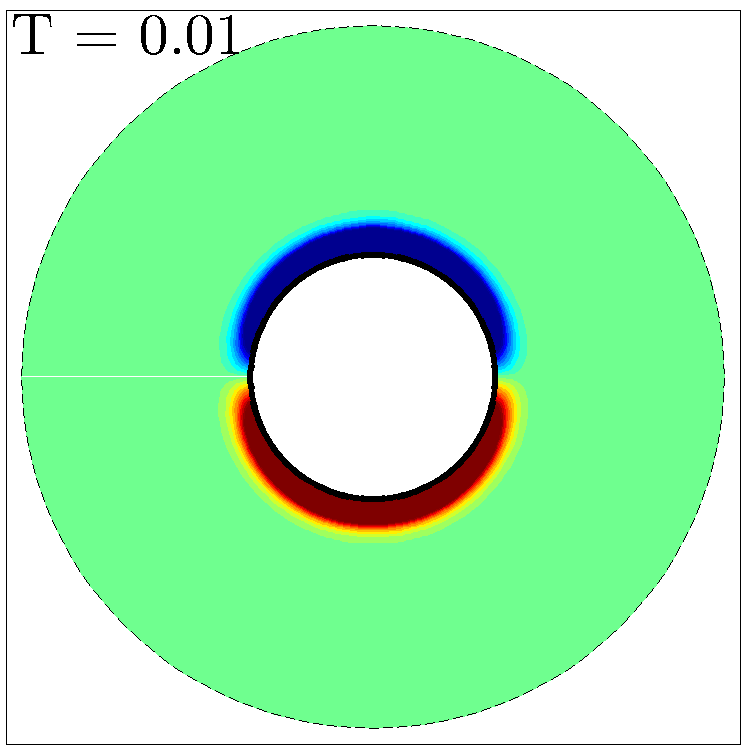
\includegraphics[width=6.5cm]{./Figures/results/static/vorticity_T0_01.pdf} & 
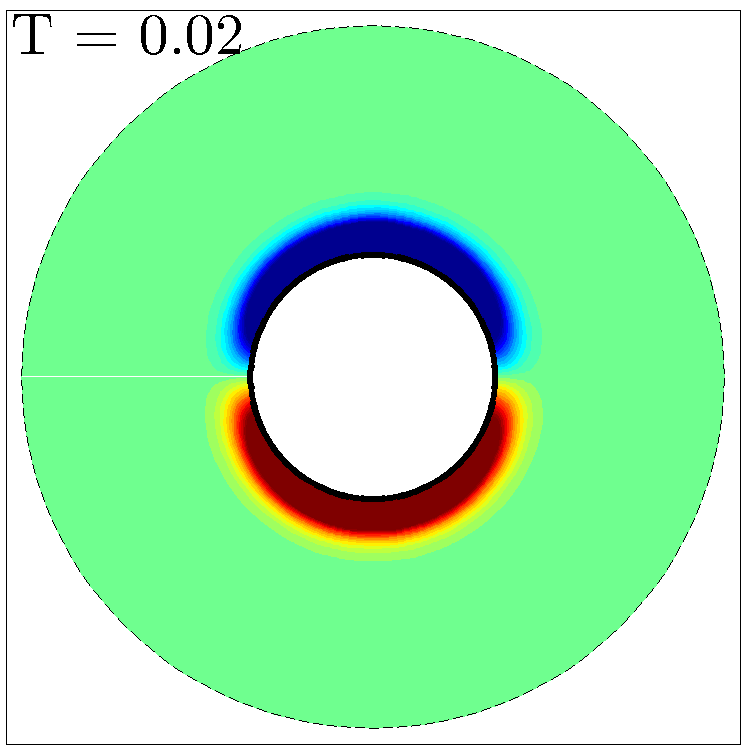
\includegraphics[width=6.5cm]{./Figures/results/static/vorticity_T0_02.pdf}  \\
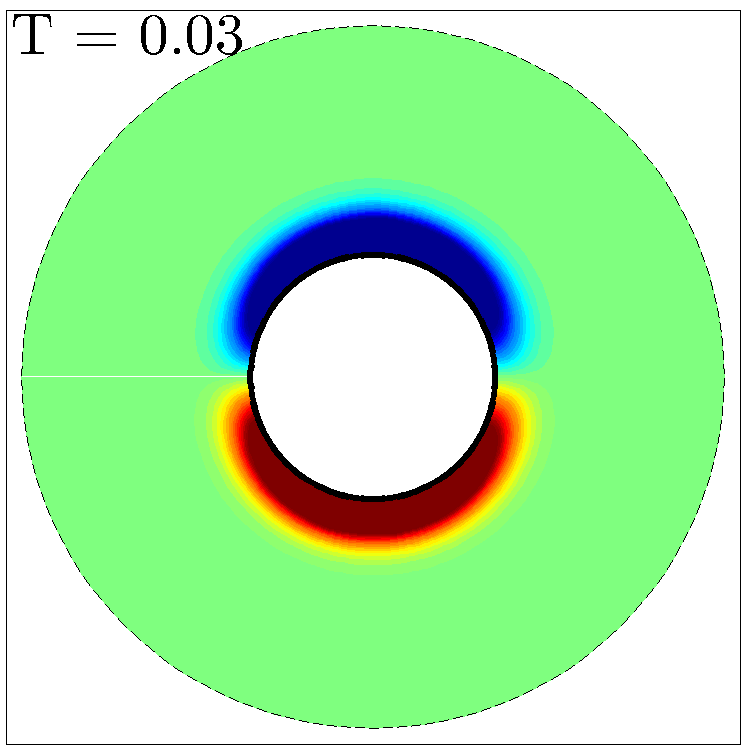
\includegraphics[width=6.5cm]{./Figures/results/static/vorticity_T0_03.pdf} & 
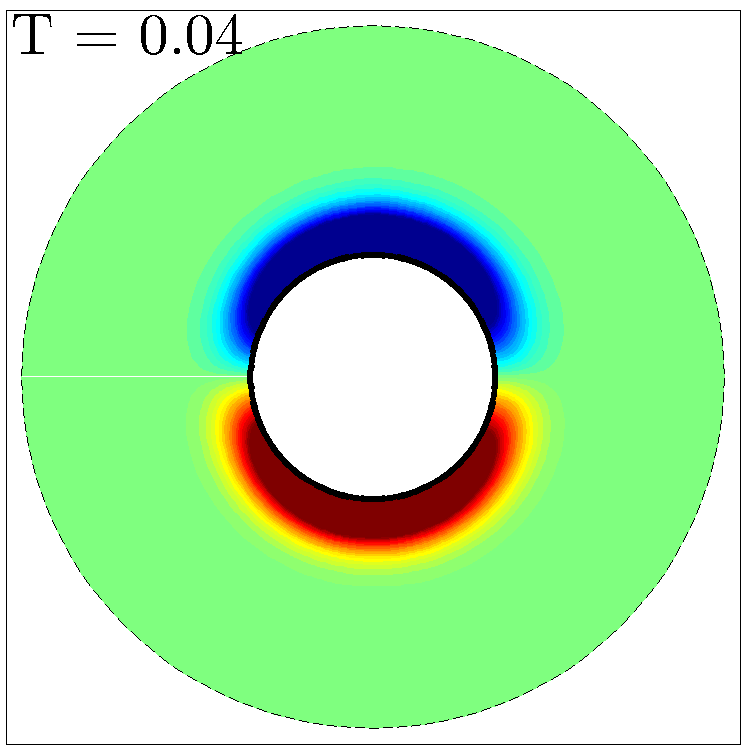
\includegraphics[width=6.5cm]{./Figures/results/static/vorticity_T0_04.pdf} \\
\end{tabular}
\end{center}
\caption[Initial vorticity development inside boundary layer]{Initial vorticity development inside boundary layer with time (boundary layer thickness magnified for visualization)}
\label{fig:InitialVorticity}
\end{figure}

\begin{figure}
\begin{center}
\begin{tabular}[t]{cc}
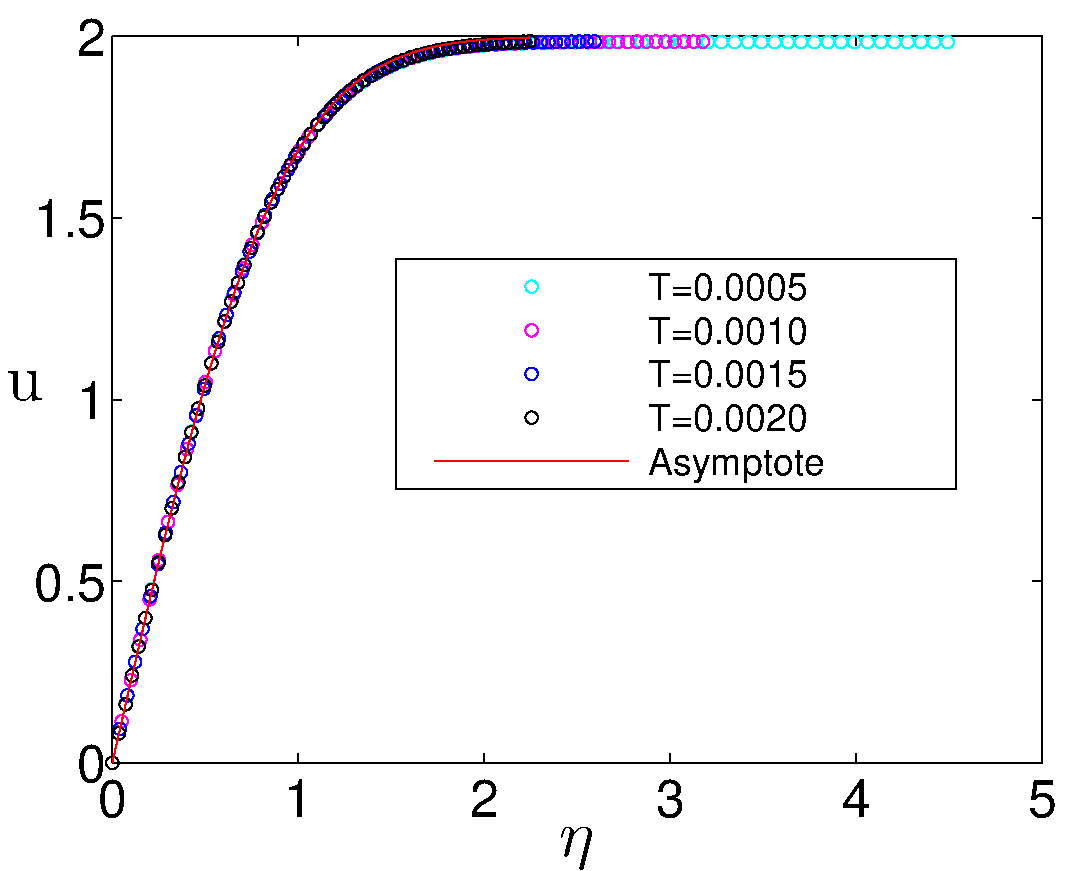
\includegraphics[width=12cm]{./Figures/results/static/u_asymptotic.pdf}  \\
(a) \\
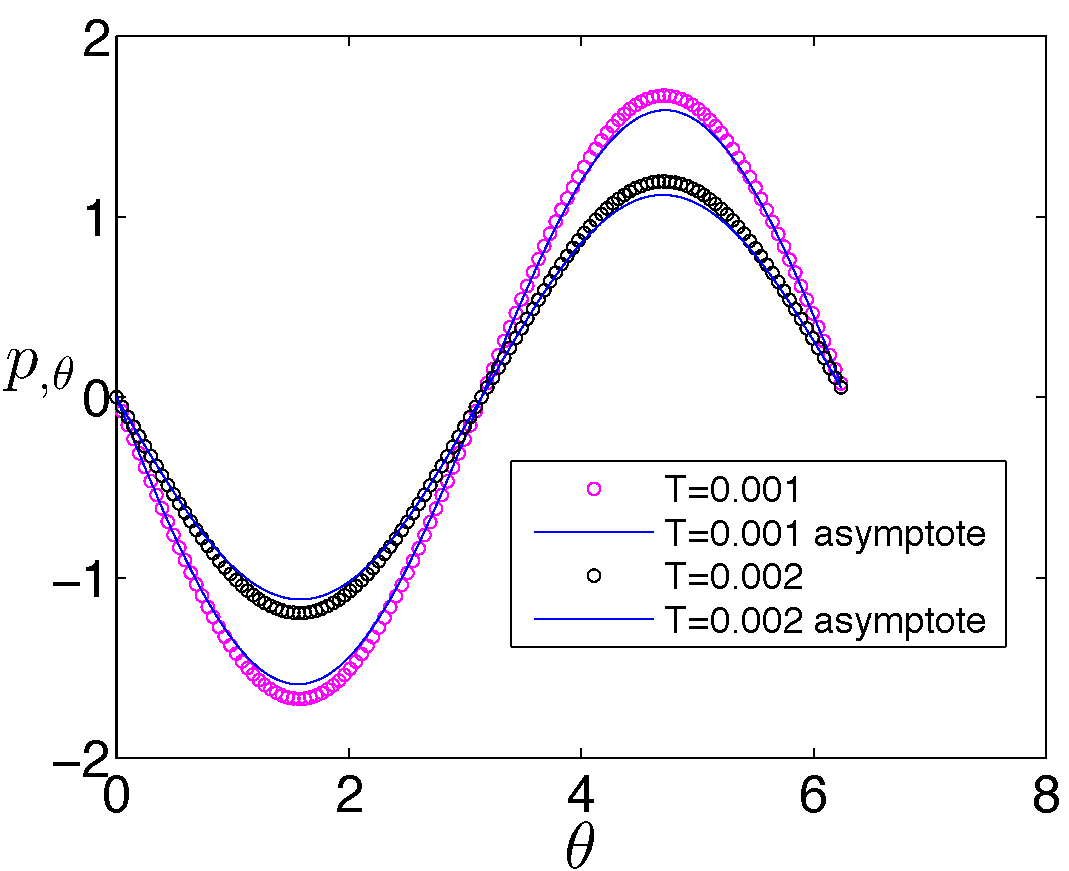
\includegraphics[width=12cm]{./Figures/results/static/p_asymptotic.pdf} \\
(b)
\end{tabular}
\end{center}
 \caption[Initial velocity and pressure inside boundary layer]{Initial flow properties compared with asymptotic solutions \cite{bar1975initial}. (a) shows that tangential velocity profiles at $\theta = \pi/2$ at different times collapse to the asymptotic solution; (b) shows the perturbation of pressure to inviscid case compared with the asymptotic solution.}
 \label{fig:InitialVelocity}
\end{figure}

\begin{figure}
\begin{center}
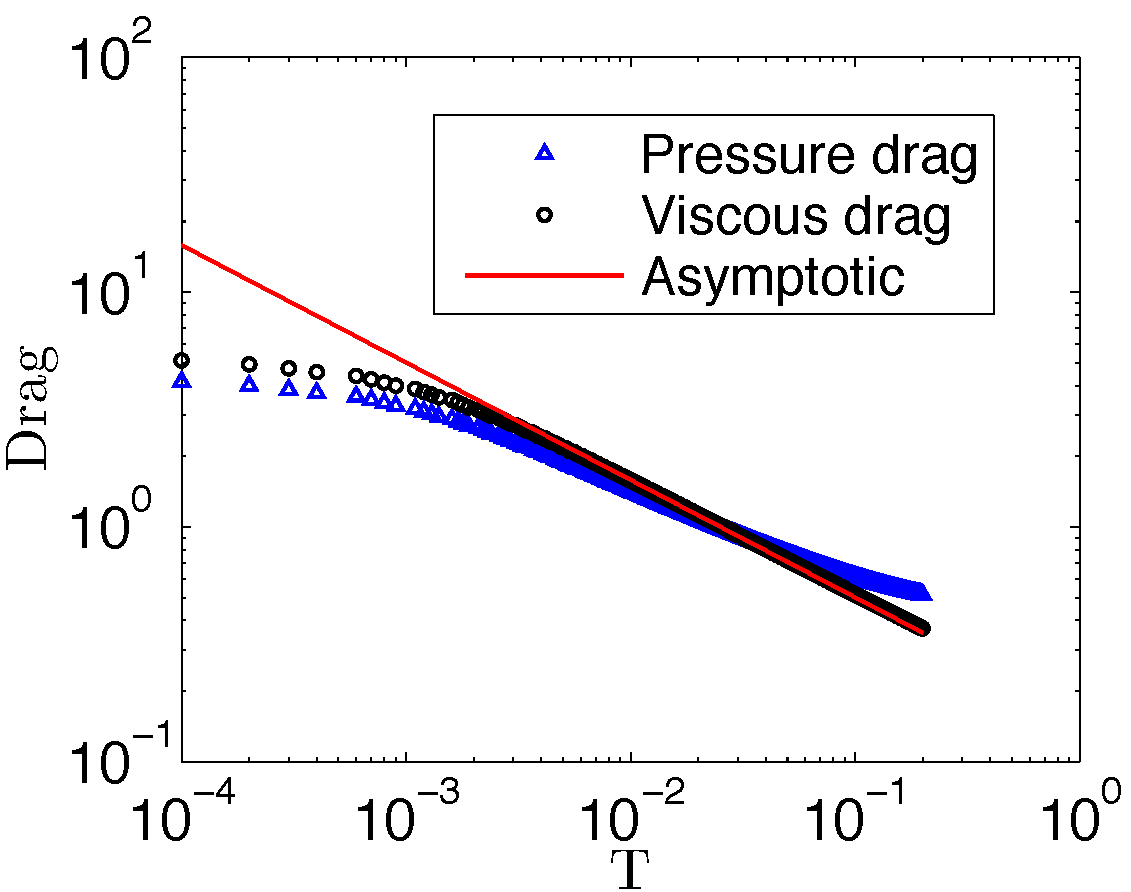
\includegraphics[width=12cm]{./Figures/results/static/InitialDrag.pdf}
\end{center}
 \caption[Initial drag coefficient]{The drag coefficients at small time compared with asymptotic solution.}
 \label{fig:InitialDrag}
\end{figure}


\subsection{Flow separation}

One important feature which enriches the phenomena is the separation of flow from the cylinder surface.
Theoretically, flow separation brings most of the difficulties to various models, including the Prandtl's boundary layer approximation which is a component of our model.
But surprisingly, except some flow details, our model captures most of the important features of the flow.
Some of the reasons behind this has been mentioned earlier in the part Rationale, and it will also be discussed later.

The separation point has several different physical definitions, and we will refer to the point at which the vorticity vanishes and the vorticity gradient along the cylinder is negative, indicating a normal flow away from the cylinder.
In that same paper, Bar-Lev \& Yang \cite{bar1975initial} obtained the following second order solution for tangential velocity
\begin{align} \label{eqn:BarLevYang2}
u =  2 erf(\eta) \sin(\theta) + 2 \sqrt{\frac{T}{Re}} f_1(\eta) \sin(\theta) + 2T f_2(\eta) \sin(2\theta),
\end{align}
with complicated functions $f_1$, $f_2$, and with these higher order terms the separation of flow is predicted.
Figure \ref{fig:Separation1} (a) and \ref{fig:Separation2} (a) show that the layer of strong vorticity separates from the cylinder surface firstly at the point close to the rear stagnation and then the separation point moves upstream with time on both sides.
On the other hand, with further diffusion and advection of vorticity, significant vorticity crosses our artificially-chosen boundary $C$ of boundary layer and discrete point vortices are shed into the outer region to represent the vorticity distribution as shown in Figure \ref{fig:Separation1} (b) and \ref{fig:Separation2} (b).
It is seen that the overall vorticity distribution is captured well, even when we switch the representation from the continuous Eulerian field inside boundary layer to the discrete Lagrangian point vortices in the outer region.

\begin{figure}
 \begin{center}
 \begin{tabular}{cc}
 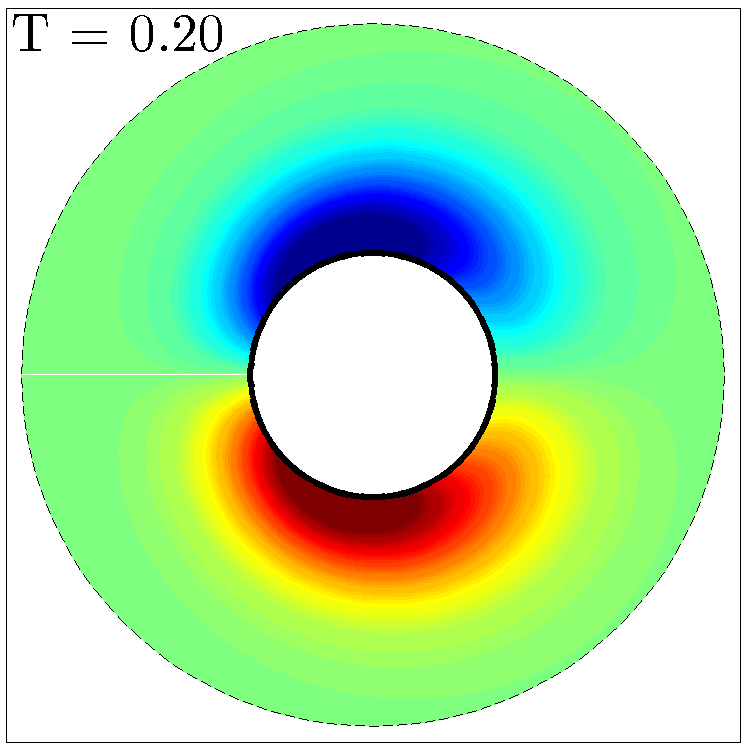
\includegraphics[height=4.5cm]{./Figures/results/static/vorticity_T0_20.pdf} &
 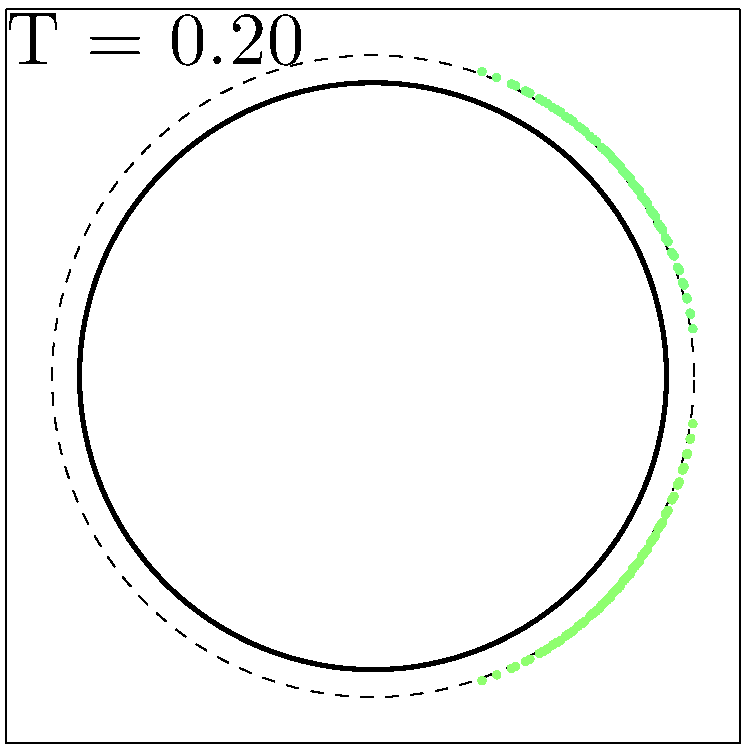
\includegraphics[height=4.5cm]{./Figures/results/static/vortices_T0_20.pdf}  \\
 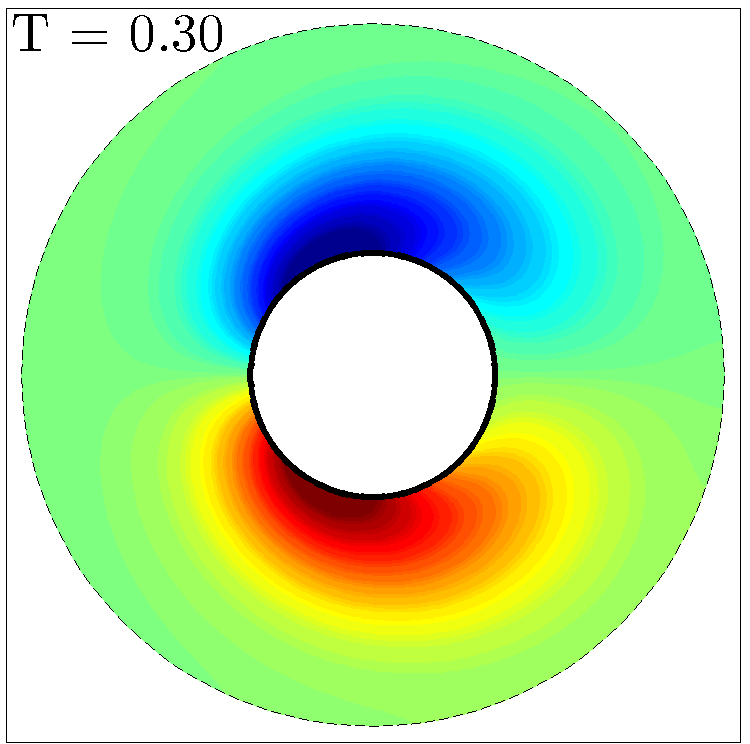
\includegraphics[height=4.5cm]{./Figures/results/static/vorticity_T0_30.pdf} &
 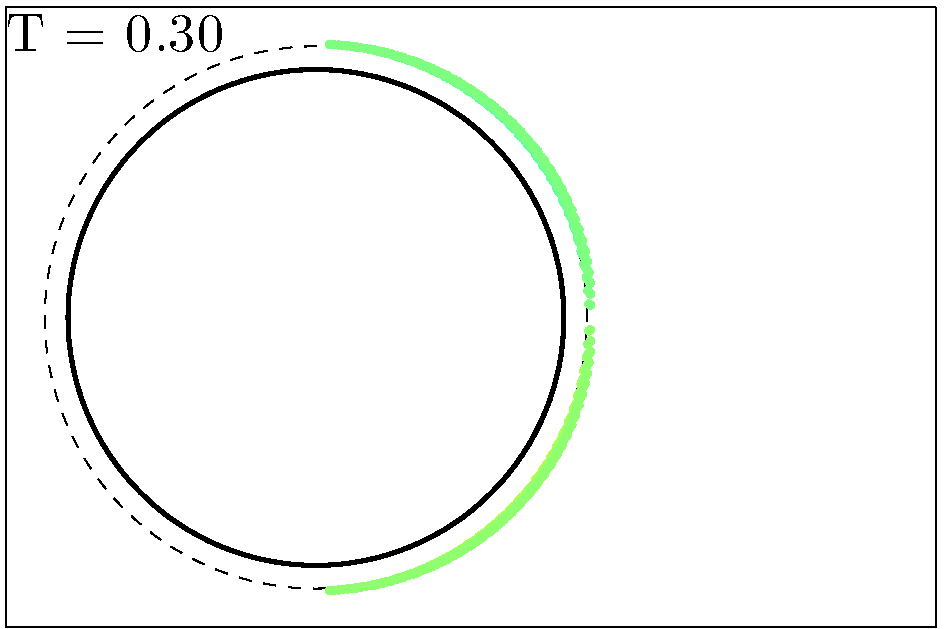
\includegraphics[height=4.5cm]{./Figures/results/static/vortices_T0_30.pdf}  \\
 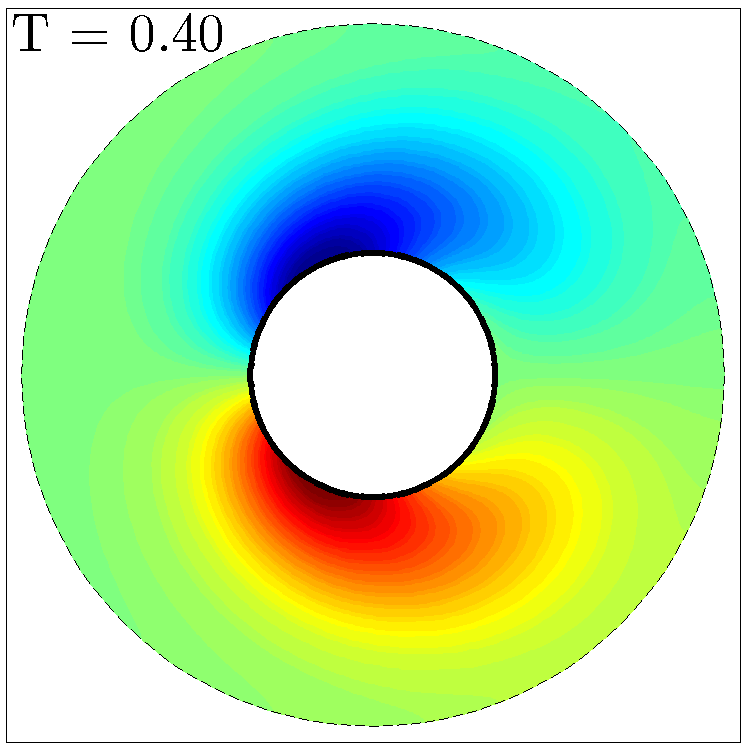
\includegraphics[height=4.5cm]{./Figures/results/static/vorticity_T0_40.pdf} &
 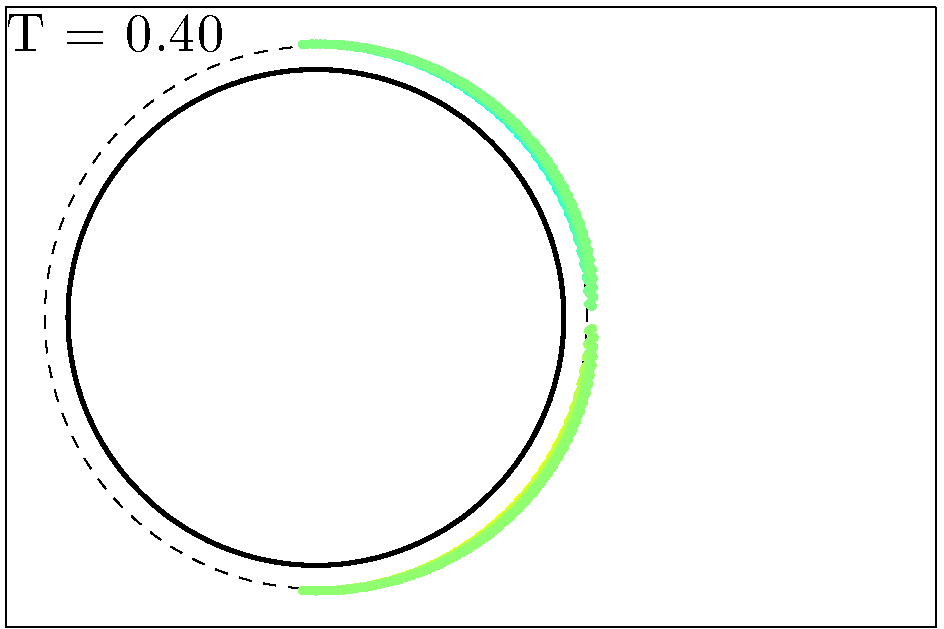
\includegraphics[height=4.5cm]{./Figures/results/static/vortices_T0_40.pdf}  \\
 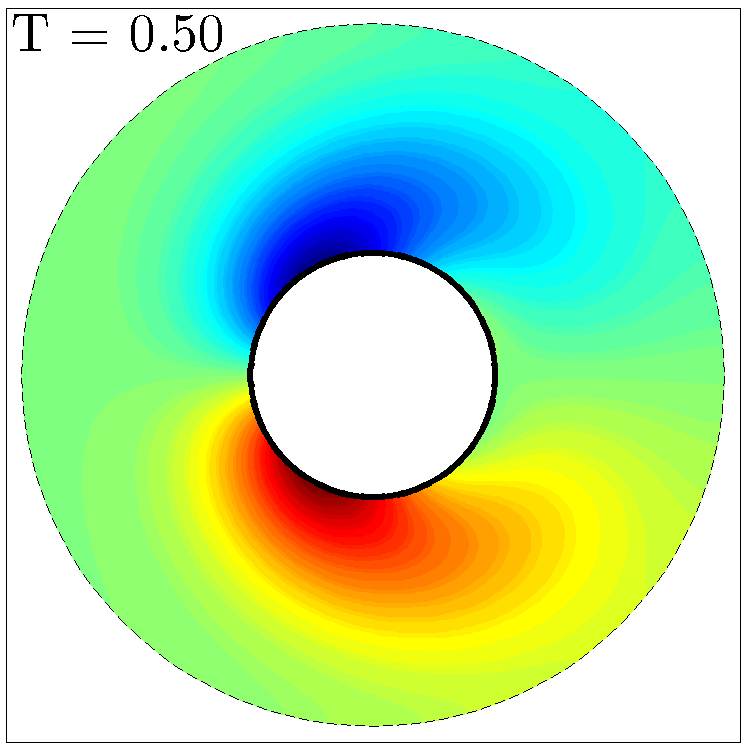
\includegraphics[height=4.5cm]{./Figures/results/static/vorticity_T0_50.pdf} &
 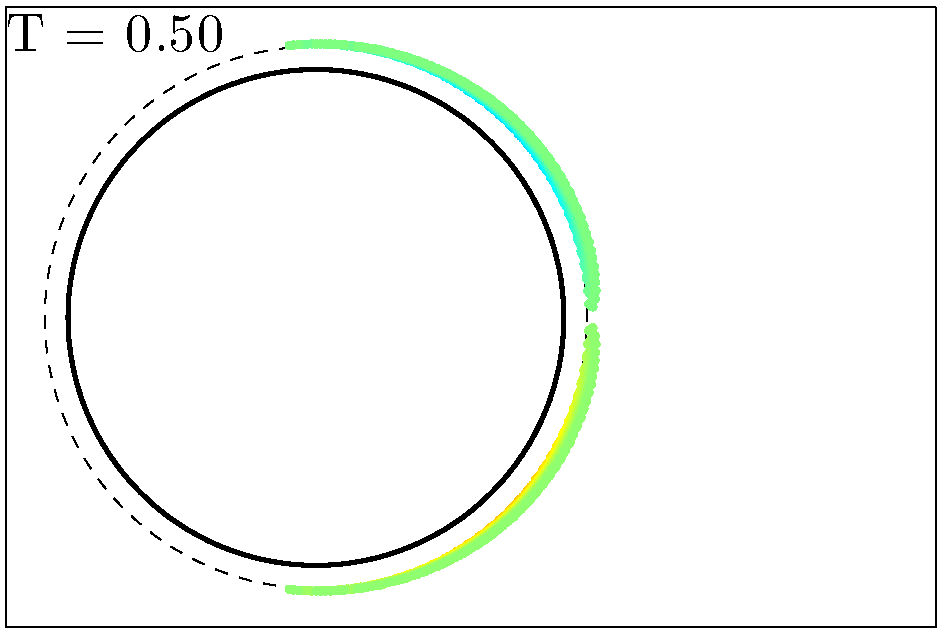
\includegraphics[height=4.5cm]{./Figures/results/static/vortices_T0_50.pdf}  \\
 (a) & (b)
\end{tabular}
\end{center}
 \caption[Flow separation shown by vorticity development]{The flow separates (a) as the vorticity gets diffused and convected away from the body for T = 0.2, 0.3, 0.4, 0.5. When significant vorticity reaches the edge of boundary layer, certain amount of point vortices are shed into the outer region (b). }
 \label{fig:Separation1}
\end{figure}

\begin{figure}
 \begin{center}
 \begin{tabular}{cc}
 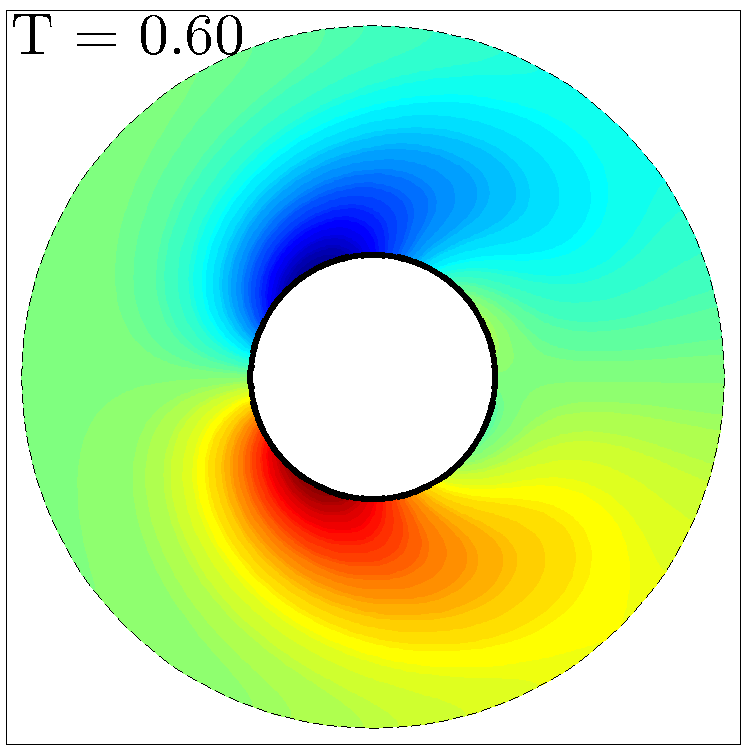
\includegraphics[height=4.5cm]{./Figures/results/static/vorticity_T0_60.pdf} &
 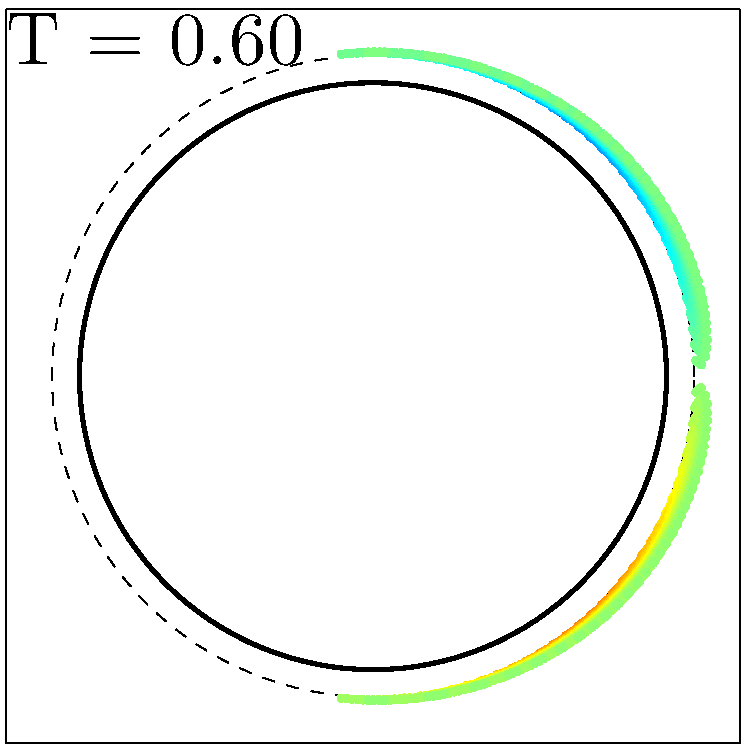
\includegraphics[height=4.5cm]{./Figures/results/static/vortices_T0_60.pdf}  \\
 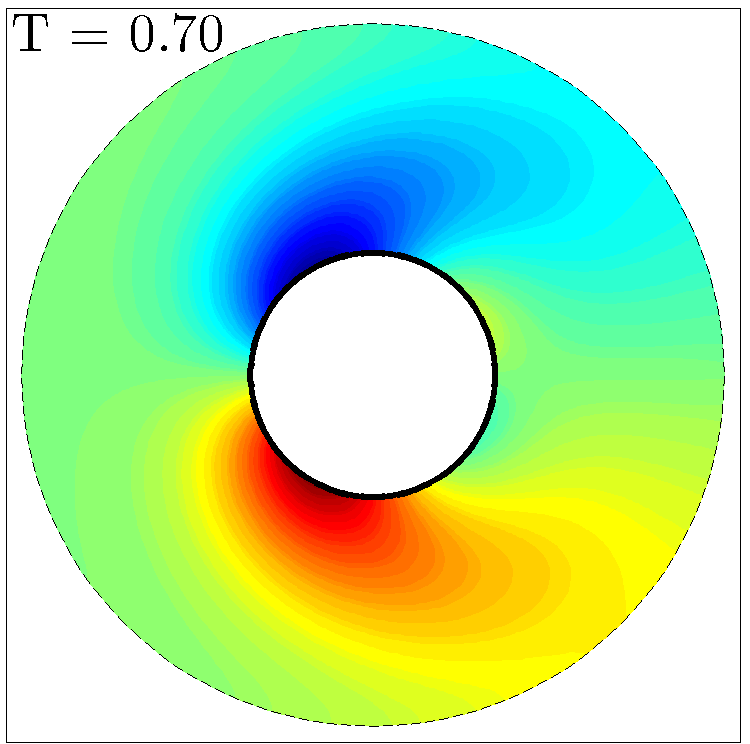
\includegraphics[height=4.5cm]{./Figures/results/static/vorticity_T0_70.pdf} &
 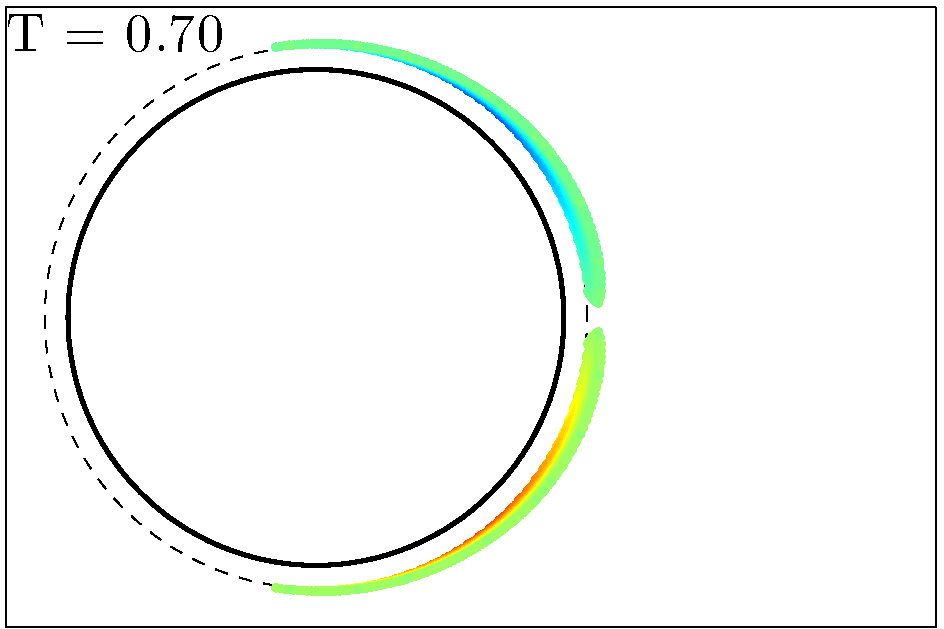
\includegraphics[height=4.5cm]{./Figures/results/static/vortices_T0_70.pdf}  \\
 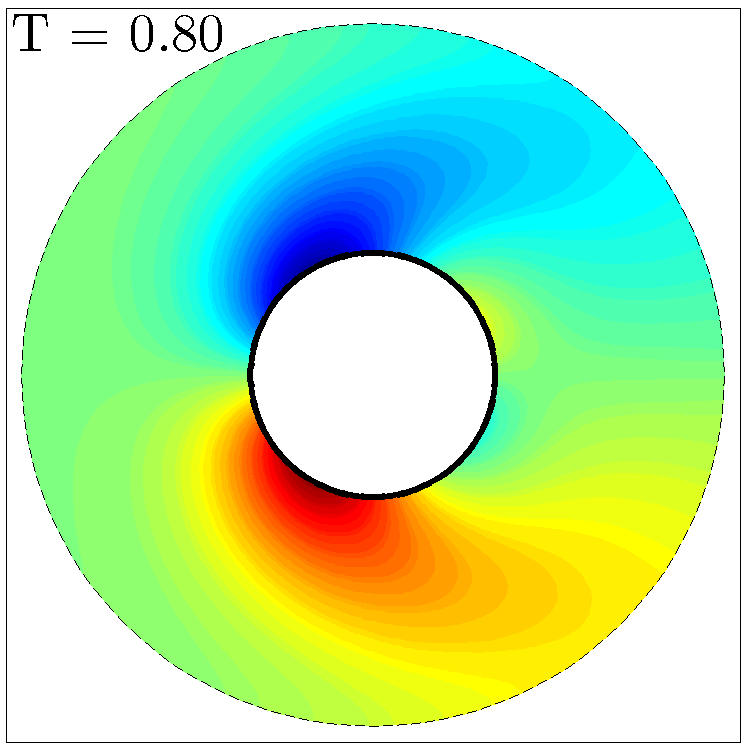
\includegraphics[height=4.5cm]{./Figures/results/static/vorticity_T0_80.pdf} &
 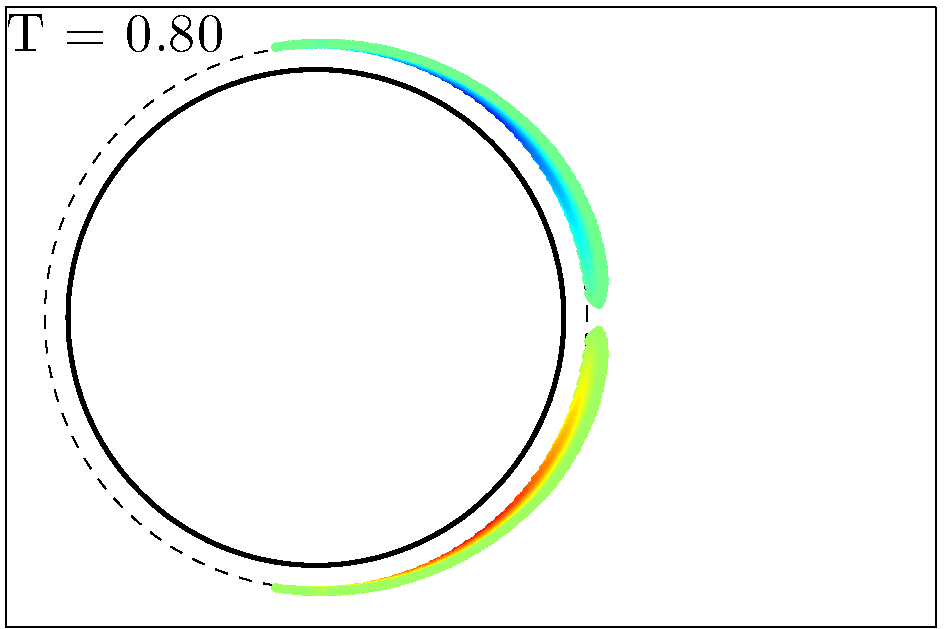
\includegraphics[height=4.5cm]{./Figures/results/static/vortices_T0_80.pdf}  \\
 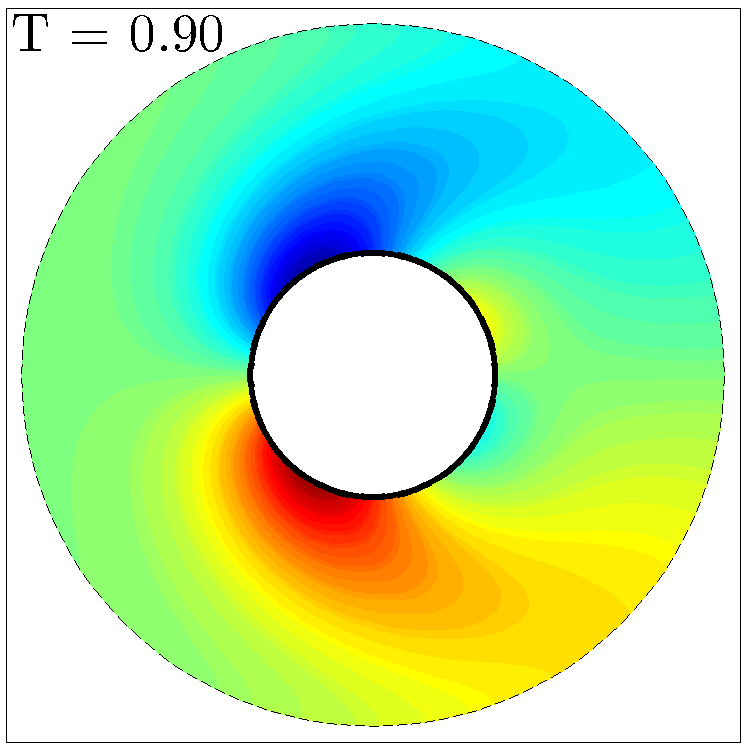
\includegraphics[height=4.5cm]{./Figures/results/static/vorticity_T0_90.pdf} &
 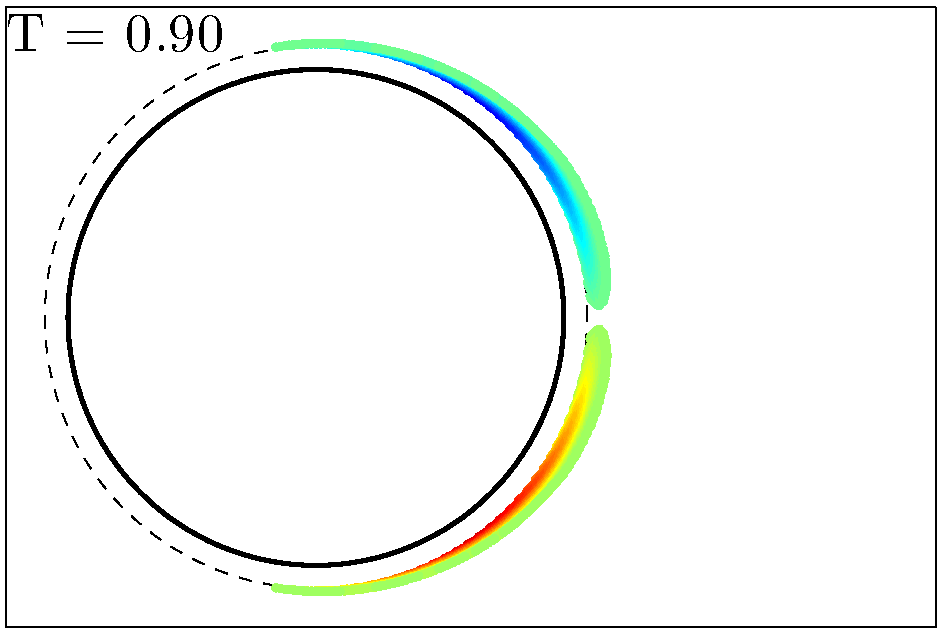
\includegraphics[height=4.5cm]{./Figures/results/static/vortices_T0_90.pdf}  \\
 (a) & (b)
\end{tabular}
\end{center}
 \caption[Flow separation shown by vorticity development]{The flow separates (a) as the vorticity gets diffused and convected away from the body for T = 0.6, 0.7, 0.8, 0.9. When significant vorticity reaches the edge of boundary layer, certain amount of point vortices are shed into the outer region (b). }
 \label{fig:Separation2}
\end{figure}

The evolution of separation point with time is quantitatively shown in Figure \ref{fig:SeparationAngle}. 
It is seen that the initial separation from the cylinder surface occurs at around $T = 0.4$, which agrees well with the asymptotic solution.
Up to $T=6$, the boundary layer has not reached a steady state yet and hopefully after longer time the separation angle will approach the correct steady value.
But it is seen that  compared to the DNS result by Koumoutsakos \& Lenoard \cite{koumoutsakos1995high} (referred as KL hereafter), our separation point moves away from the rear stagnation point slower.
This phenomena (and some others shown later) might be due to numerics. 
When the vortices get convected backwards from the unstructured outer region to the structured boundary layer, they might not be completely absorbed, which leads to an incomplete capture of the recirculation effect. 

\begin{figure}
 \begin{center}
 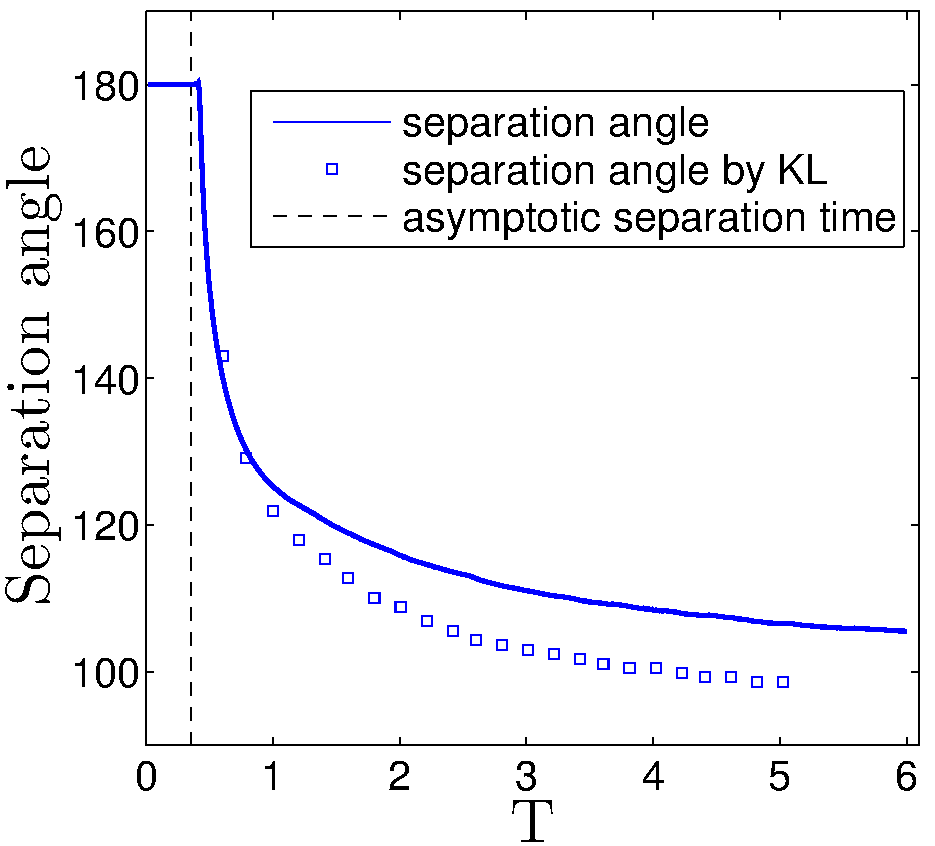
\includegraphics[width=12cm]{./Figures/results/static/separation_angle.pdf}
 \end{center}
 \caption[Evolution of separation angle]{The time progression of separation angle compared with the direct numerical simulation result by KL \cite{koumoutsakos1995high}.}
 \label{fig:SeparationAngle}
\end{figure}


\subsection{Vortex shedding pattern in the wake}

The later-time progression of the vorticity field is shown in Figures \ref{fig:Wake1} and \ref{fig:Wake1}, with comparison to the DNS results using vortex methods \cite{koumoutsakos1995high}.
At this stage of moderate time up to $T = 6$, the wake remains symmetric,  characterized by one primary vortex and one small secondary vortex on both upper and lower half planes. 
Fed by a thick shear layer connected to the body, each primary vortex is passively convected by the free-stream velocity.
Initially the layer that feeds the primary vortex changes angle of orientation in respect to the body, but it seems that a stable configuration is in place later.
As the secondary vortex grows, it penetrates the primary vortex but it is always confined and never able to reach the outer irrotational flow field.
Compared to the result by KL \cite{koumoutsakos1995high}, the feeding vorticity layer is spanning a smaller angle relative to the body, indicating a little bit weaker vortex shedding, and this could also partially explain why the separation angle predicted by our model moves away from the rear point slower than that predicted by KL \cite{koumoutsakos1995high}.


\begin{figure}
 \begin{center}
 \begin{tabular}{cc}
 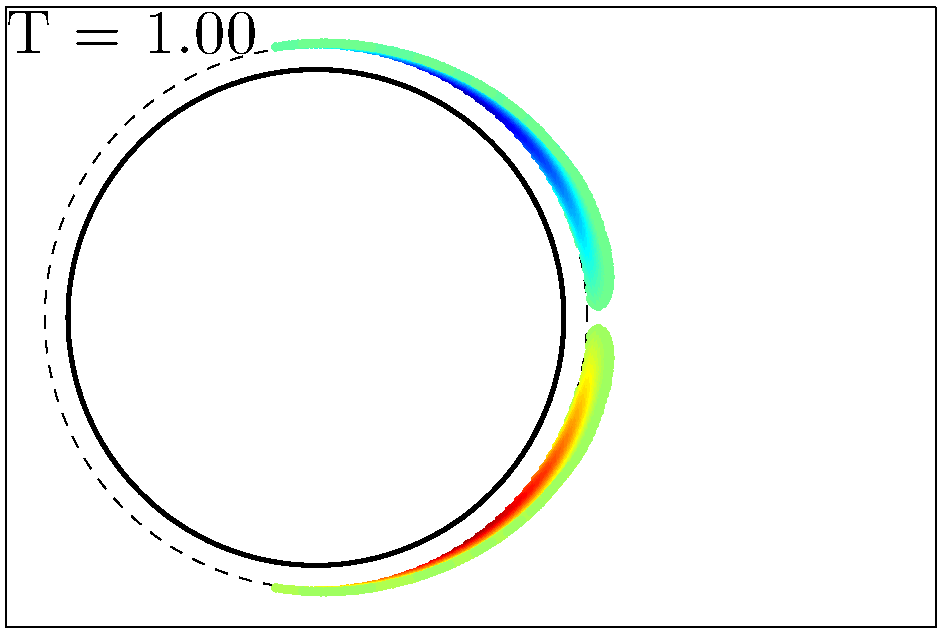
\includegraphics[width=6.5cm]{./Figures/results/static/vortices_T1_00.pdf}  &
 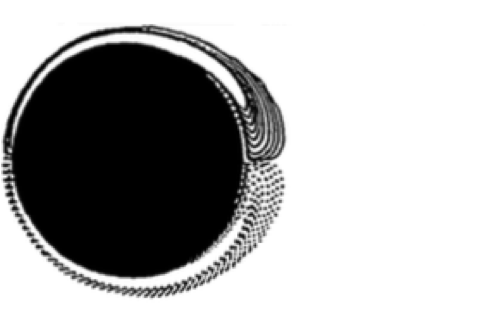
\includegraphics[width=6.5cm]{./Figures/results/static/KOU_Re1000_T1.png}  \\
 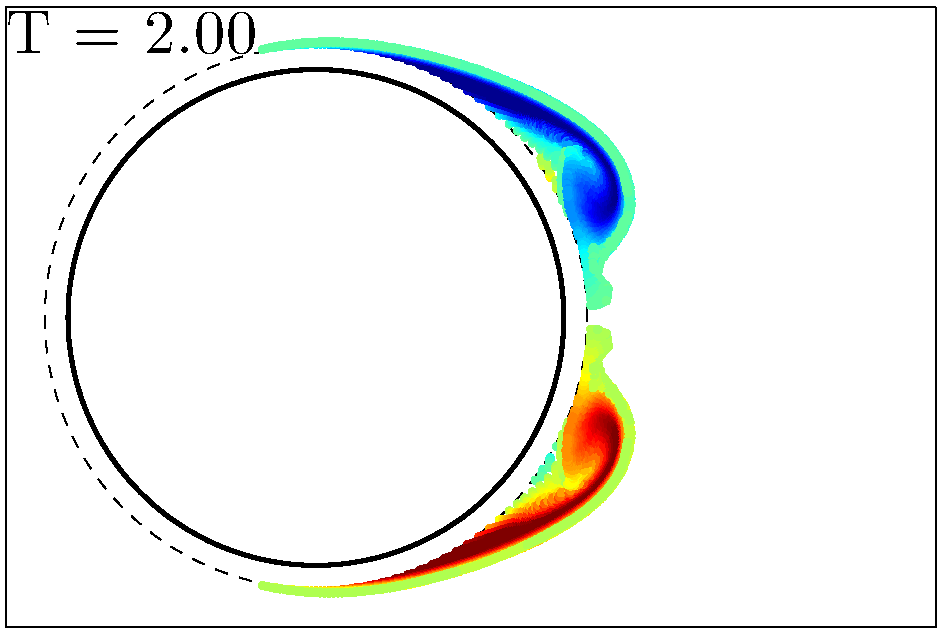
\includegraphics[width=6.5cm]{./Figures/results/static/vortices_T2_00.pdf}  &
 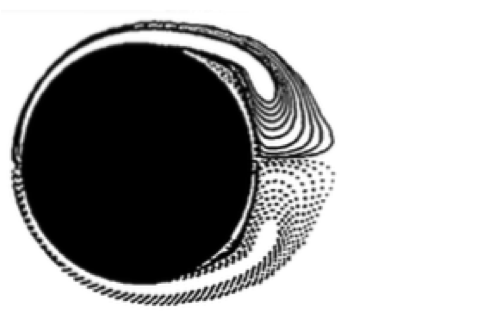
\includegraphics[width=6.5cm]{./Figures/results/static/KOU_Re1000_T2.png}  \\
 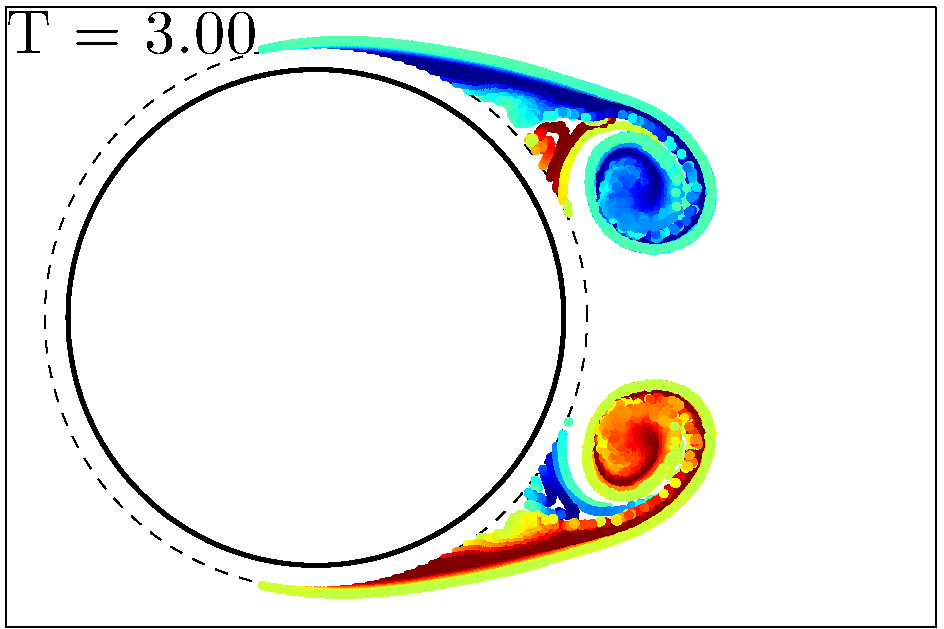
\includegraphics[width=6.5cm]{./Figures/results/static/vortices_T3_00.pdf}  &
 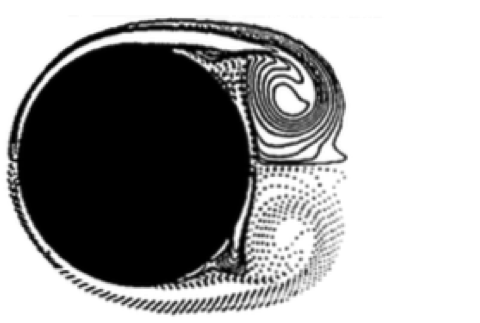
\includegraphics[width=6.5cm]{./Figures/results/static/KOU_Re1000_T3.png}  \\
 (a) & (b) \\
 \end{tabular}
\end{center}
 \caption[Vortex shedding pattern in the wake]{The progression of vortex shedding pattern (a) with comparison to direct numerical simulation result by vortex methods (b) for T = 1, 2, 3. }
 \label{fig:Wake1}
\end{figure}

\begin{figure}
 \begin{center}
 \begin{tabular}{cc}
 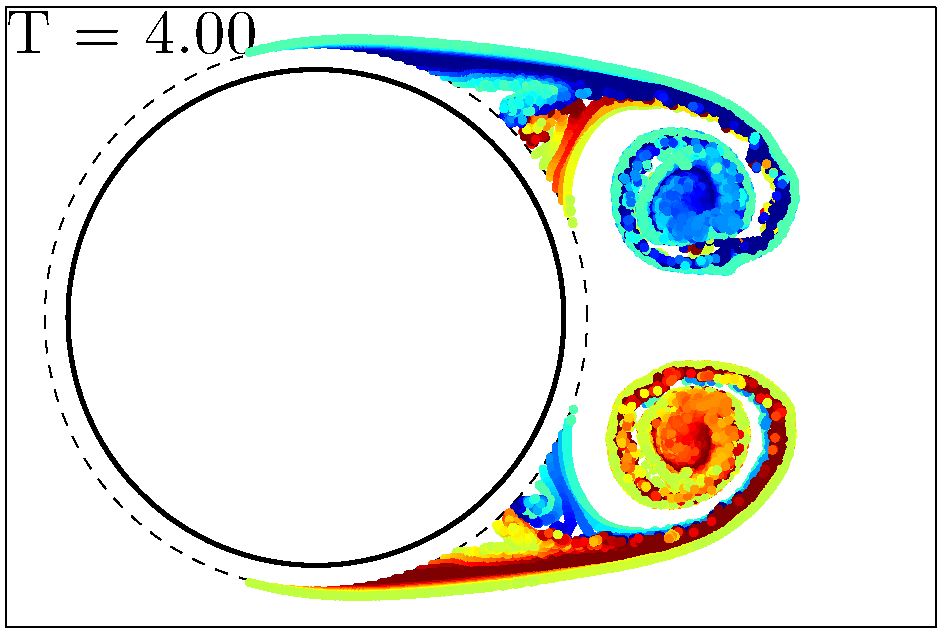
\includegraphics[width=6.5cm]{./Figures/results/static/vortices_T4_00.pdf}  &
 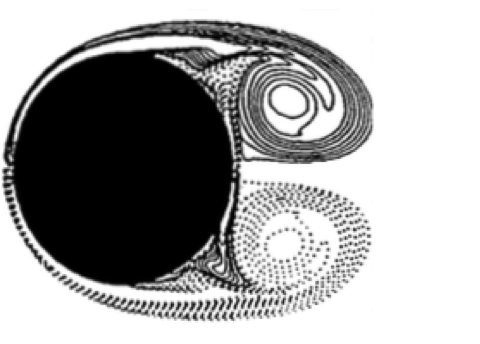
\includegraphics[width=6.5cm]{./Figures/results/static/KOU_Re1000_T4.png}  \\
 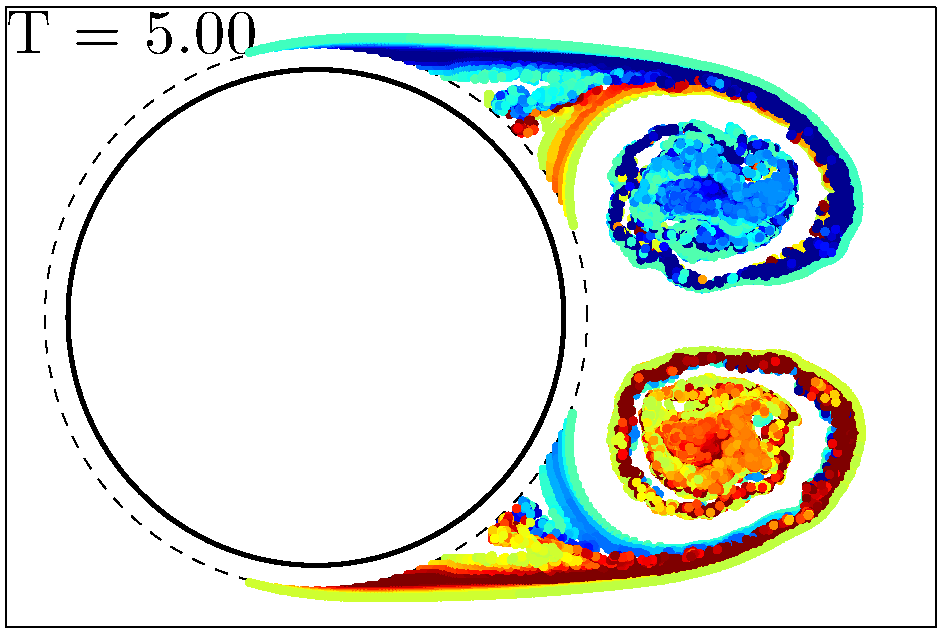
\includegraphics[width=6.5cm]{./Figures/results/static/vortices_T5_00.pdf}  &
 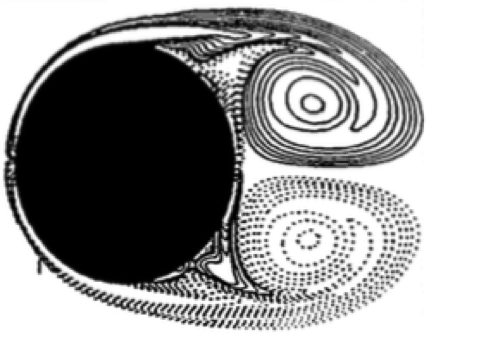
\includegraphics[width=6.5cm]{./Figures/results/static/KOU_Re1000_T5.png}  \\
 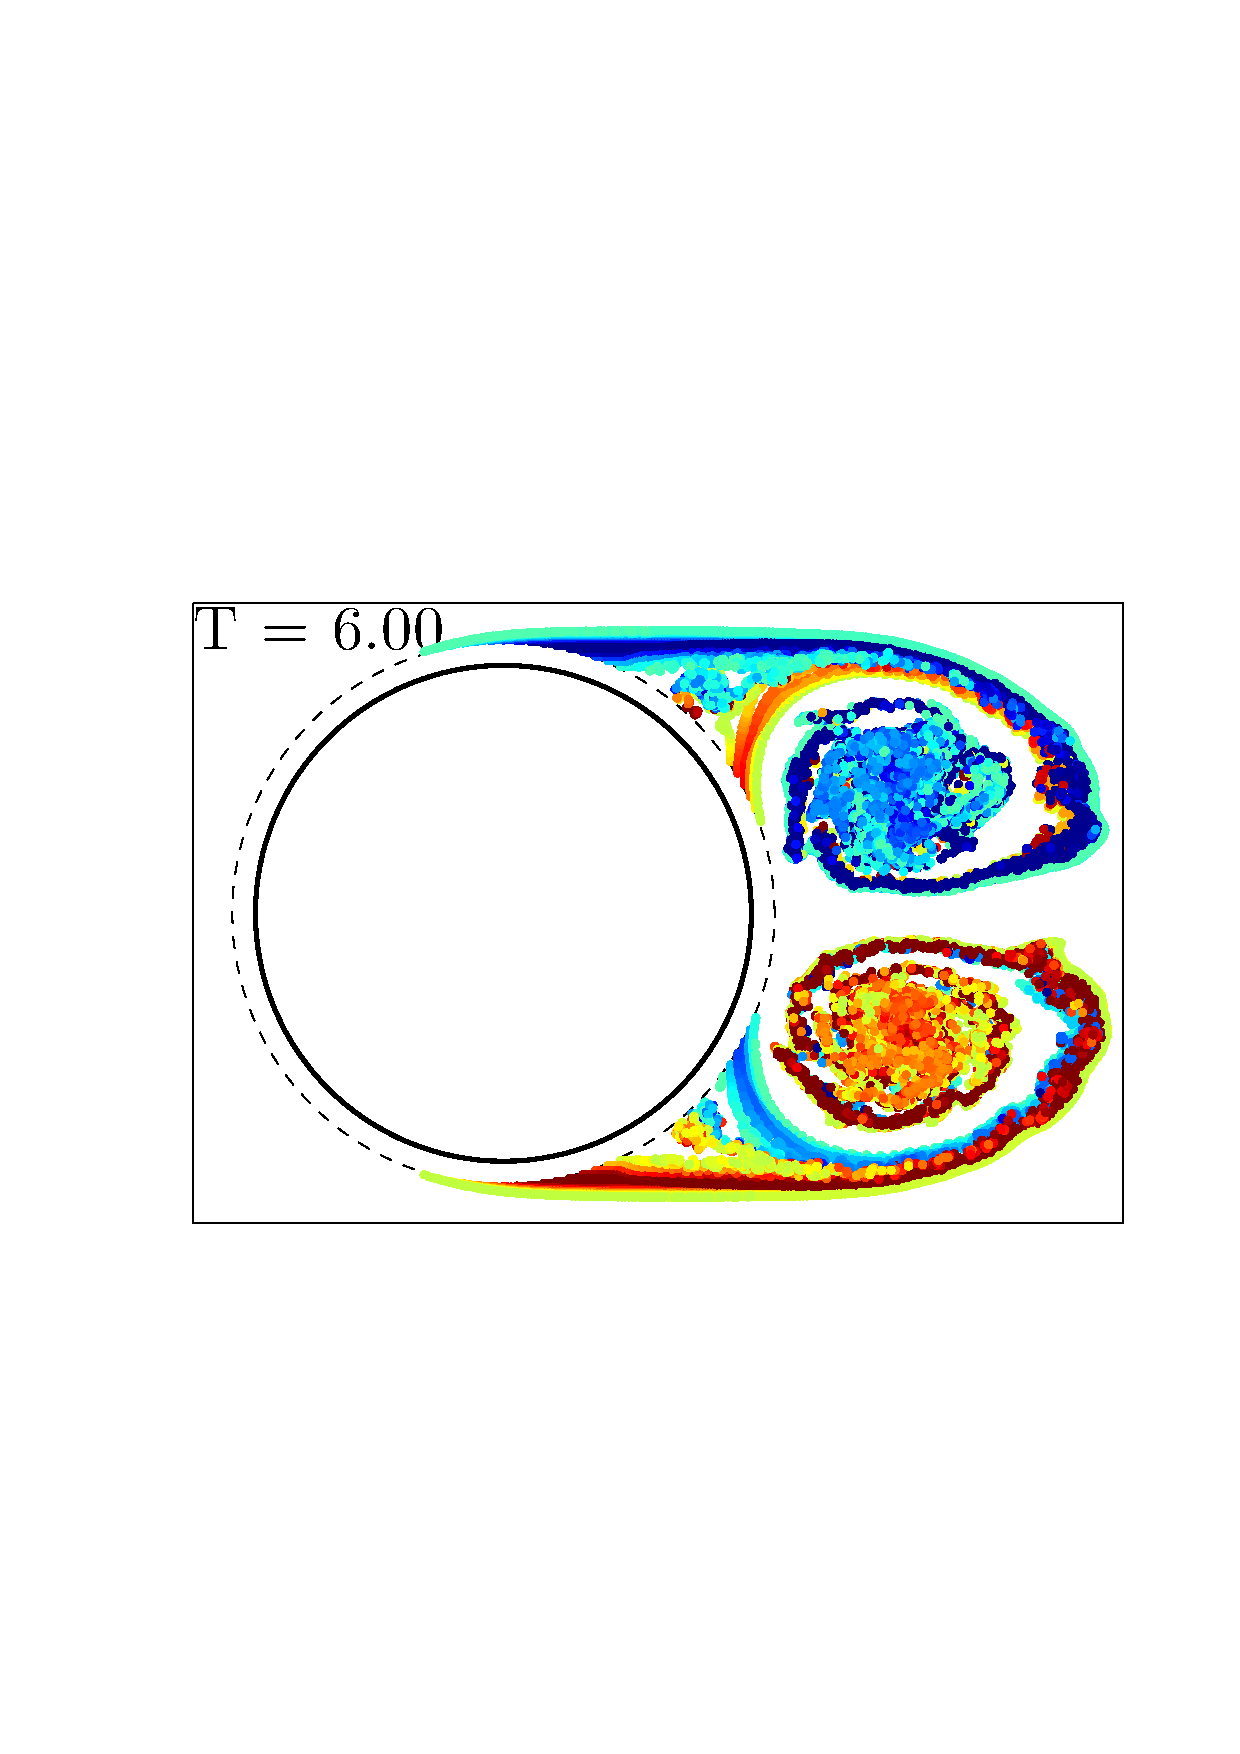
\includegraphics[width=6.5cm]{./Figures/results/static/vortices_T6_00.pdf}  &
 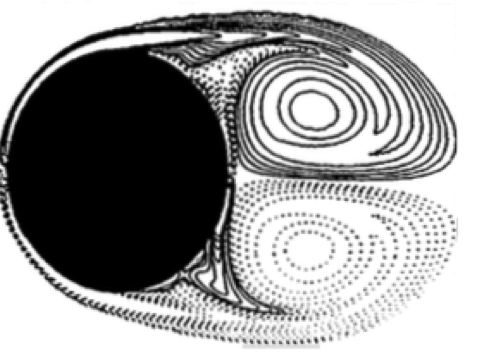
\includegraphics[width=6.5cm]{./Figures/results/static/KOU_Re1000_T6.png}  \\
 (a) & (b) \\
 \end{tabular}
\end{center}
 \caption[Vortex shedding pattern in the wake]{The progression of vortex shedding pattern (a) with comparison to direct numerical simulation result by vortex methods (b) for T = 4, 5, 6. }
 \label{fig:Wake2}
\end{figure}

One of the most important quantitative features to observe here is still the drag coefficient, which is shown in Figure \ref{fig:Drag}.
It's seen that the viscous drag agrees well with the DNS result by KL, following the correct asymptote $2\sqrt{\pi/ReT}$.
On the other hand, the pressure drag is predicted with the same trend as that by KL, but quantitatively our pressure drag is higher than theirs.
The reason behind this might still be related to the fact mentioned earlier that we didn't quite capture the circulation in the rear completely.

\begin{figure}
\begin{center}
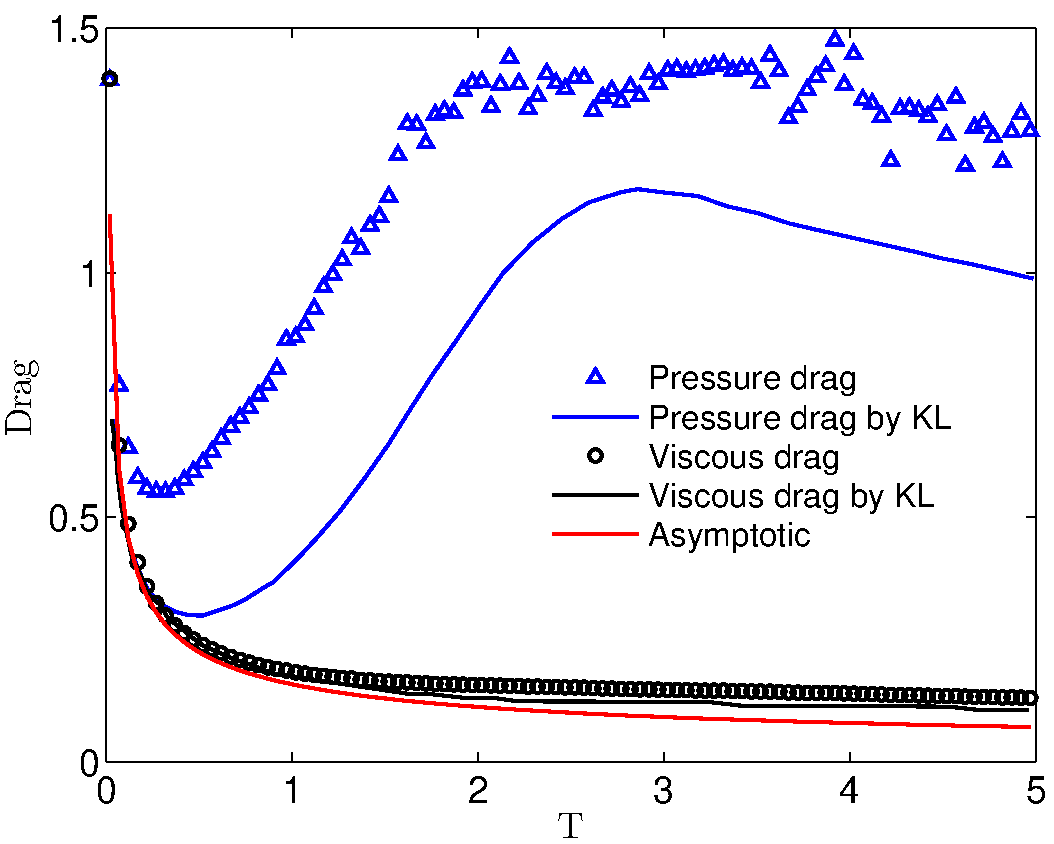
\includegraphics[width=12cm]{./Figures/results/static/Drag.pdf}
\end{center}
\caption[Drag coefficient]{The drag coefficient compared with direct numerical simulation results and small-time asymptotic.}
\label{fig:Drag}
\end{figure}


\subsection{Irrelevance of boundary layer thickness}

Last but not least, although Prandtl's boundary layer approximation is expected to fail at the separation point, we still believe that our model can capture the vortex shedding.
One of the important arguments we have behind the belief is that even with the separation occurring the solution will still reach an asymptote as the distance from the body increases, and  the solution should not depend on the precise boundary layer thickness within certain precision as long as we switch the representation at a reasonable place.
To partially confirm this, the total circulation in the upper-half plane (due to symmetry) computed with different boundary layer thickness $c/\sqrt{Re}$ is shown in Figure \ref{fig:Circulation}.
For comparison, the circulation calculated by DNS is also plotted.
It is clearly seen that the circulation predicted by our model qualitatively follows the same trend as the DNS result.
Besides, it confirms  that within certain range the exact location of the interface $C$ does not affect the total circulation significantly, but just determines where we switch over the representation of flows.

\begin{figure}
\begin{center}
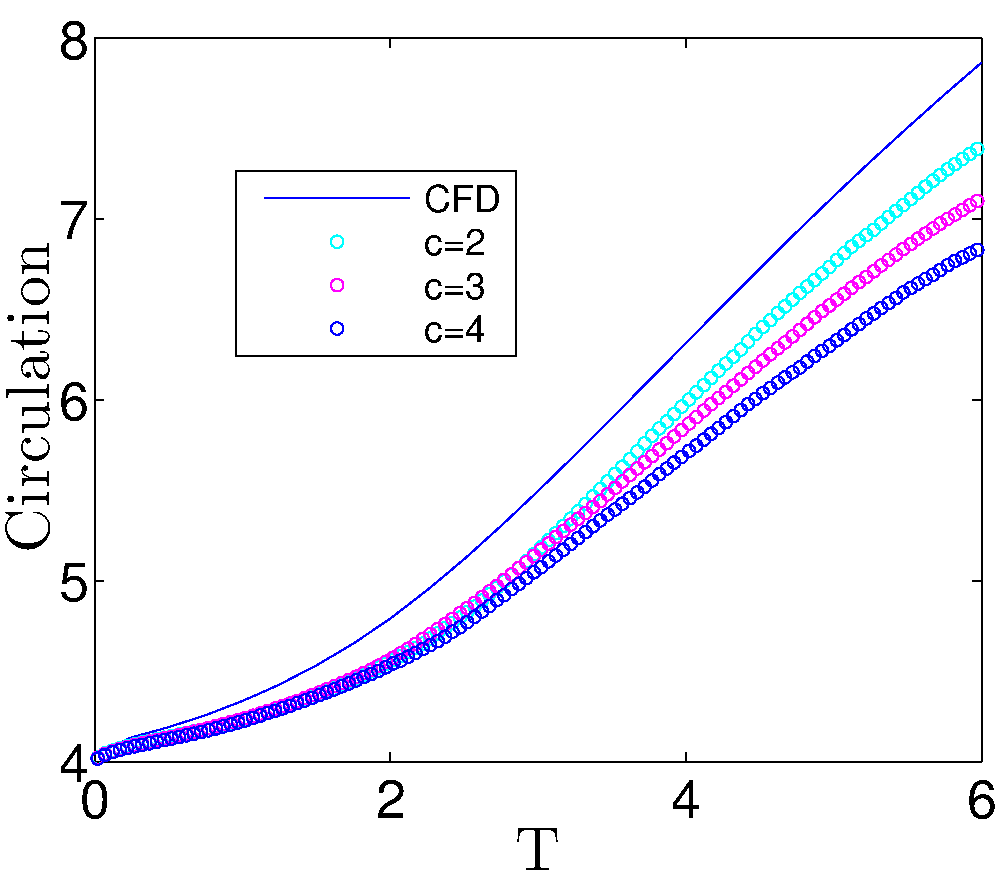
\includegraphics[width=12cm]{./Figures/results/static/Circulation.pdf}
\end{center}
\caption[Total circulation in the upper-half plane]{Total circulation in the upper-half plane calculated with different boundary layer thickness $c/\sqrt{Re}$, compared with CFD result.}
\label{fig:Circulation}
\end{figure}


\section{Impulsively started flow past a sinusoidally rotating cylinder}

\noindent \\
\tikz \draw (0, 0) rectangle (\linewidth, 3in) node[pos=0.3]{Introduction to this problem};


\noindent \\
\tikz \draw (0, 0) rectangle (\linewidth, 3in) node[pos=0.3]{Discussion about the result};


\begin{figure}
 \begin{center}
 \begin{tabular}{cc}
 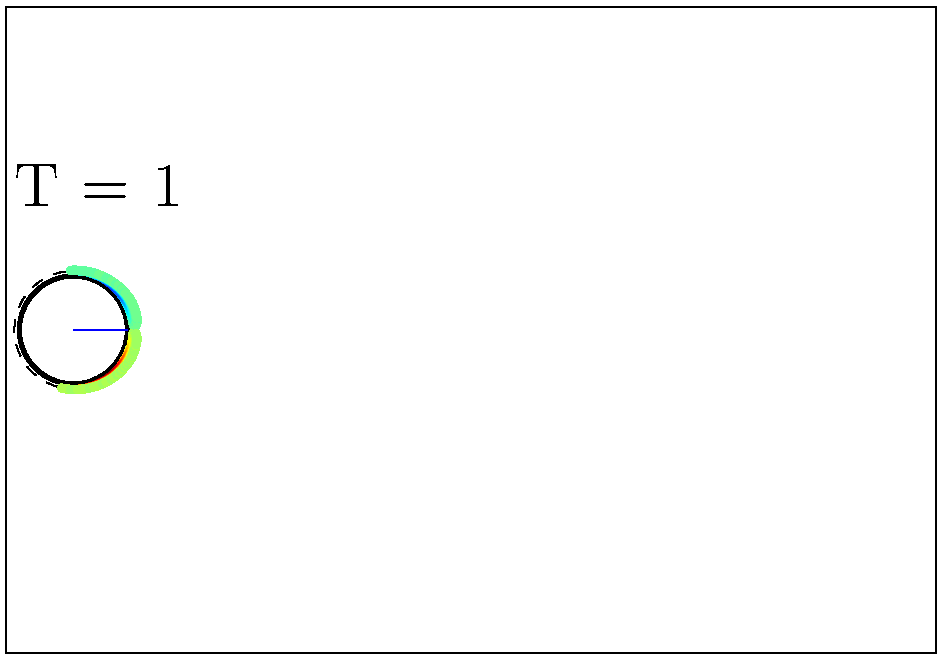
\includegraphics[height=4.5cm]{./Figures/results/rotating/vortices_T1.pdf}  &
 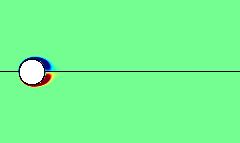
\includegraphics[height=4.5cm]{./Figures/results/rotating/T_1.png}  \\
 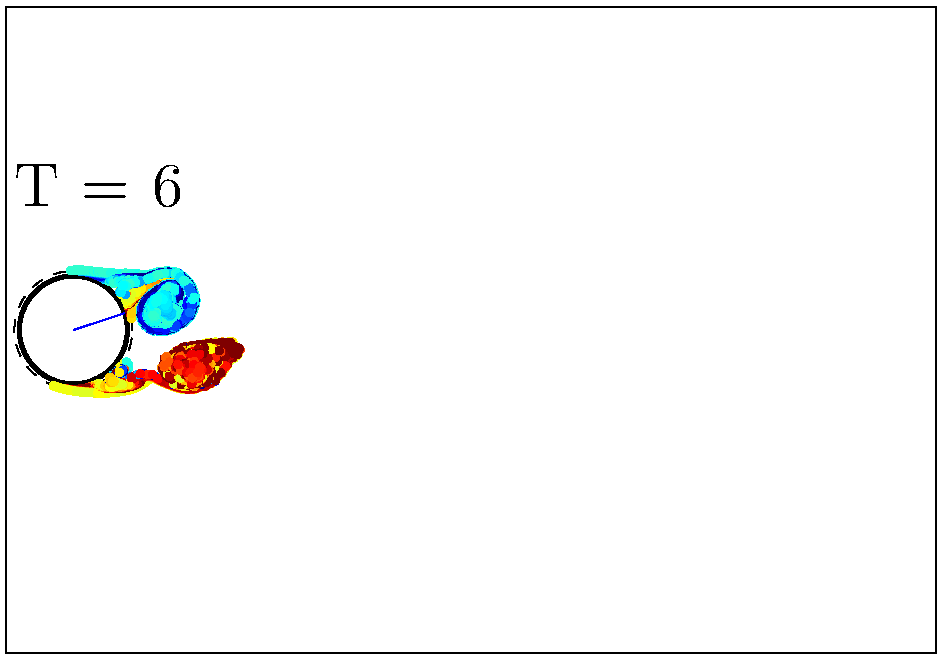
\includegraphics[height=4.5cm]{./Figures/results/rotating/vortices_T6.pdf}  &
 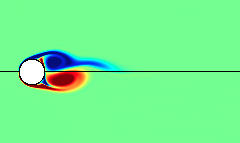
\includegraphics[height=4.5cm]{./Figures/results/rotating/T_6.png}  \\
 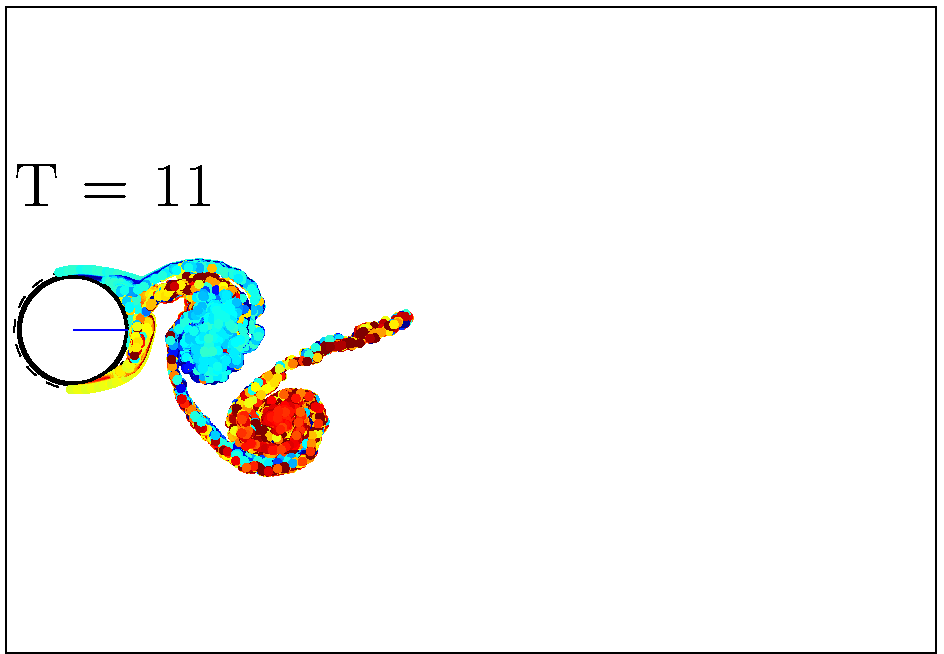
\includegraphics[height=4.5cm]{./Figures/results/rotating/vortices_T11.pdf}  &
 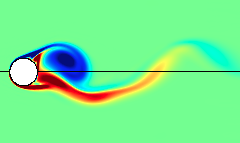
\includegraphics[height=4.5cm]{./Figures/results/rotating/T_11.png}  \\
 (a) & (b) \\
 \end{tabular}
\end{center}
 \caption[Vortex shedding pattern around a sinusoidally rotating cylinder]{The progression of vortex shedding pattern (a) with comparison to direct numerical simulation result (b) for T = 1, 6, 11. }
 \label{fig:RotatingWake1}
\end{figure}

\begin{figure}
 \begin{center}
 \begin{tabular}{cc}
 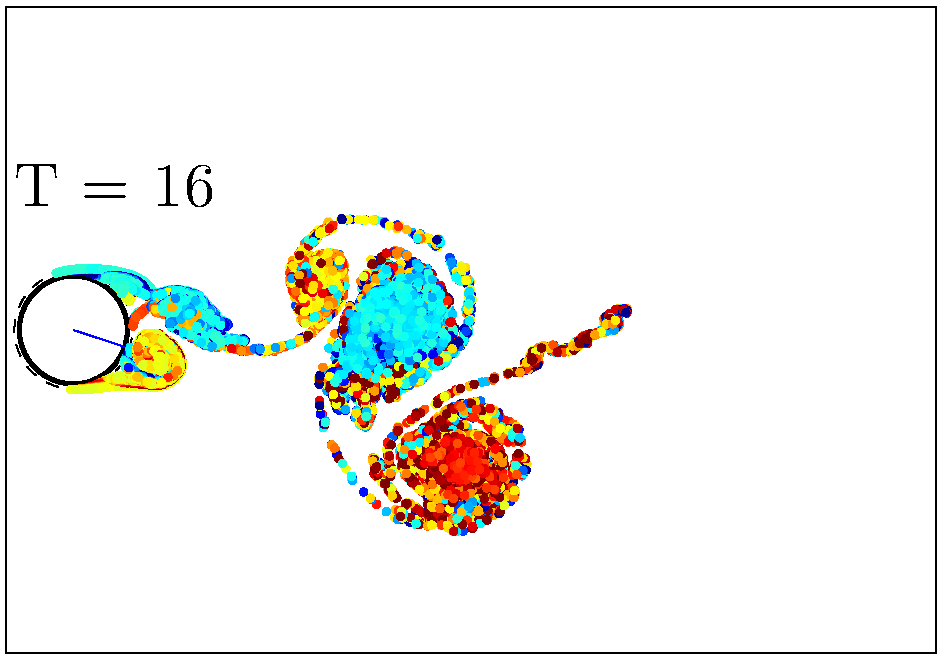
\includegraphics[height=4.5cm]{./Figures/results/rotating/vortices_T16.pdf}  &
 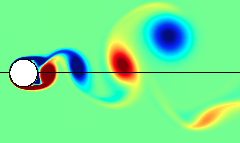
\includegraphics[height=4.5cm]{./Figures/results/rotating/T_16.png}  \\
 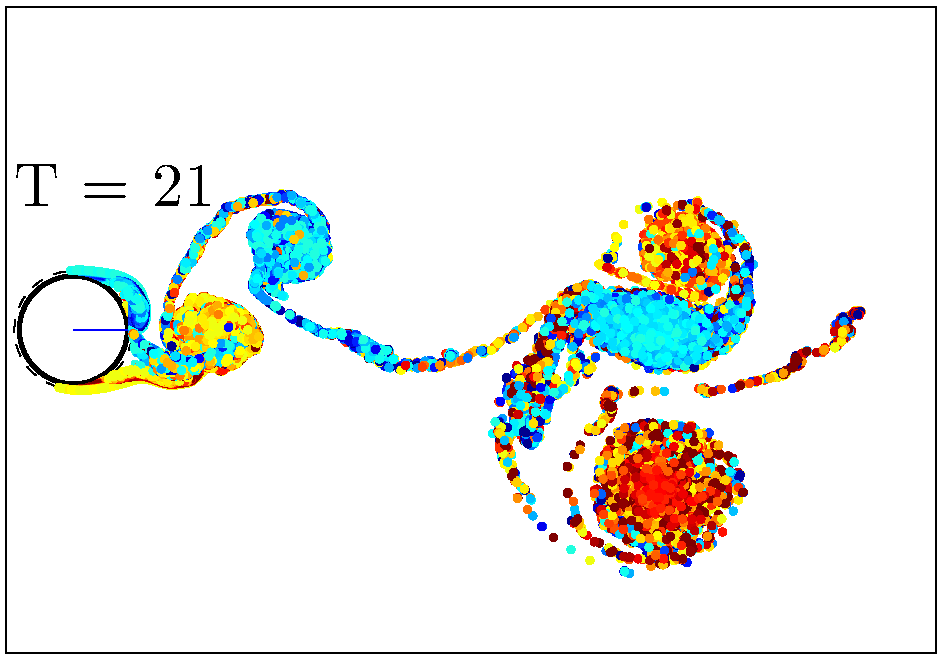
\includegraphics[height=4.5cm]{./Figures/results/rotating/vortices_T21.pdf}  &
 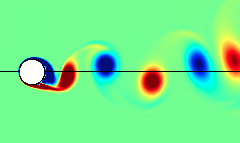
\includegraphics[height=4.5cm]{./Figures/results/rotating/T_21.png}  \\
 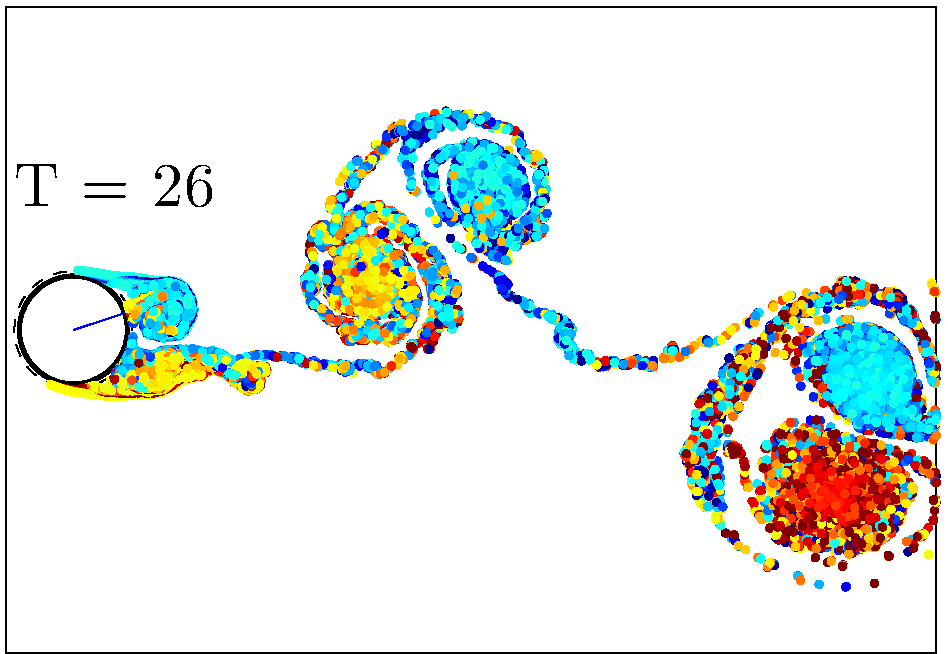
\includegraphics[height=4.5cm]{./Figures/results/rotating/vortices_T26.pdf}  &
 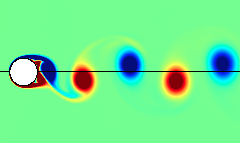
\includegraphics[height=4.5cm]{./Figures/results/rotating/T_26.png}  \\
 (a) & (b) \\
 \end{tabular}
\end{center}
 \caption[Vortex shedding pattern around a sinusoidally rotating cylinder]{The progression of vortex shedding pattern (a) with comparison to direct numerical simulation result (b) for T = 16, 21, 26. }
 \label{fig:RotatingWake2}
\end{figure}

